\documentclass{beamer}
\usetheme{tokitex}

\usepackage{tikz}
\usepackage{graphics}
\usepackage{multirow}
\usepackage{tabto}
\usepackage{xspace}
\usepackage{amsmath}
\usepackage{hyperref}
\usepackage{wrapfig}
\usepackage{mathtools}

\usepackage{tikz}
\usepackage{clrscode3e}
\usepackage{gensymb}

\usepackage[english,bahasa]{babel}
\newtranslation[to=bahasa]{Section}{Bagian}
\newtranslation[to=bahasa]{Subsection}{Subbagian}

\usepackage{listings, lstautogobble}
\usepackage{color}

\definecolor{dkgreen}{rgb}{0,0.6,0}
\definecolor{gray}{rgb}{0.5,0.5,0.5}
\definecolor{mauve}{rgb}{0.58,0,0.82}

\lstset{frame=tb,
  language=c++,
  aboveskip=0mm,
  belowskip=0mm,
  showstringspaces=false,
  columns=fullflexible,
  keepspaces=true,
  basicstyle={\small\ttfamily},
  numbers=none,
  numberstyle=\tiny\color{gray},
  keywordstyle=\color{blue},
  commentstyle=\color{dkgreen},
  stringstyle=\color{mauve},
  breaklines=true,
  breakatwhitespace=true,
  lineskip={-3pt}
}

\usepackage{caption}
\captionsetup[figure]{labelformat=empty}

\newcommand{\progTerm}[1]{\textbf{#1}}
\newcommand{\foreignTerm}[1]{\textit{#1}}
\newcommand{\newTerm}[1]{\alert{\textbf{#1}}}
\newcommand{\emp}[1]{\alert{#1}}
\newcommand{\statement}[1]{"#1"}

\newcommand{\floor}[1]{\lfloor #1 \rfloor}
\newcommand{\ceil}[1]{\lceil #1 \rceil}
\newcommand{\abs}[1]{\left\lvert#1\right\rvert}
\newcommand{\norm}[1]{\left\lVert#1\right\rVert}

% Getting tired of writing \foreignTerm all the time
\newcommand{\farray}{\foreignTerm{array}\xspace}
\newcommand{\fArray}{\foreignTerm{Array}\xspace}
\newcommand{\foverhead}{\foreignTerm{overhead}\xspace}
\newcommand{\fOverhead}{\foreignTerm{Overhead}\xspace}
\newcommand{\fsubarray}{\foreignTerm{subarray}\xspace}
\newcommand{\fSubarray}{\foreignTerm{Subarray}\xspace}
\newcommand{\fbasecase}{\foreignTerm{base case}\xspace}
\newcommand{\fBasecase}{\foreignTerm{Base case}\xspace}
\newcommand{\ftopdown}{\foreignTerm{top-down}\xspace}
\newcommand{\fTopdown}{\foreignTerm{Top-down}\xspace}
\newcommand{\fbottomup}{\foreignTerm{bottom-up}\xspace}
\newcommand{\fBottomup}{\foreignTerm{Bottom-up}\xspace}
\newcommand{\fpruning}{\foreignTerm{pruning}\xspace}
\newcommand{\fPruning}{\foreignTerm{Pruning}\xspace}

\newcommand{\fgraph}{\foreignTerm{graph}\xspace}
\newcommand{\fGraph}{\foreignTerm{Graph}\xspace}
\newcommand{\froot}{\foreignTerm{root}\xspace}
\newcommand{\fRoot}{\foreignTerm{Root}\xspace}
\newcommand{\fnode}{\foreignTerm{node}\xspace}
\newcommand{\fNode}{\foreignTerm{Node}\xspace}
\newcommand{\fedge}{\foreignTerm{edge}\xspace}
\newcommand{\fEdge}{\foreignTerm{Edge}\xspace}
\newcommand{\fcycle}{\foreignTerm{cycle}\xspace}
\newcommand{\fCycle}{\foreignTerm{Cycle}\xspace}
\newcommand{\fdegree}{\foreignTerm{degree}\xspace}
\newcommand{\fDegree}{\foreignTerm{Degree}\xspace}
\newcommand{\fadjacencylist}{\foreignTerm{adjacency list}\xspace}
\newcommand{\fAdjacencylist}{\foreignTerm{Adjacency list}\xspace}
\newcommand{\fadjacencymatrix}{\foreignTerm{adjacency matrix}\xspace}
\newcommand{\fAdjacencymatrix}{\foreignTerm{Adjacency matrix}\xspace}
\newcommand{\fedgelist}{\foreignTerm{edge list}\xspace}
\newcommand{\fEdgelist}{\foreignTerm{Edge list}\xspace}
\newcommand{\flist}{\foreignTerm{list}\xspace}
\newcommand{\fList}{\foreignTerm{List}\xspace}
\newcommand{\fgraphtraversal}{\foreignTerm{graph traversal}\xspace}
\newcommand{\fGraphtraversal}{\foreignTerm{Graph traversal}\xspace}
\newcommand{\ftree}{\foreignTerm{tree}\xspace}
\newcommand{\fTree}{\foreignTerm{Tree}\xspace}
\newcommand{\fsubtree}{\foreignTerm{subtree}\xspace}
\newcommand{\fSubtree}{\foreignTerm{Subtree}\xspace}
\newcommand{\fparent}{\foreignTerm{parent}\xspace}
\newcommand{\fParent}{\foreignTerm{Parent}\xspace}
\newcommand{\fsibling}{\foreignTerm{sibling}\xspace}
\newcommand{\fSibling}{\foreignTerm{Sibling}\xspace}
\newcommand{\fpath}{\foreignTerm{path}\xspace}
\newcommand{\fPath}{\foreignTerm{Path}\xspace}
\newcommand{\fconnectedcomponent}{\foreignTerm{connected component}\xspace}
\newcommand{\fConnectedcomponent}{\foreignTerm{Connected component}\xspace}
\newcommand{\fbridge}{\foreignTerm{bridge}\xspace}
\newcommand{\fBridge}{\foreignTerm{Bridge}\xspace}
\newcommand{\farticulationpoint}{\foreignTerm{articulation point}\xspace}
\newcommand{\fArticulationpoint}{\foreignTerm{Articulation point}\xspace}
\newcommand{\ftreeedge}{\foreignTerm{tree edge}\xspace}
\newcommand{\fTreeedge}{\foreignTerm{Tree edge}\xspace}
\newcommand{\fbackedge}{\foreignTerm{back edge}\xspace}
\newcommand{\fBackedge}{\foreignTerm{Back edge}\xspace}
\newcommand{\fforwardedge}{\foreignTerm{forward edge}\xspace}
\newcommand{\fForwardedge}{\foreignTerm{Forward edge}\xspace}
\newcommand{\fcrossedge}{\foreignTerm{cross edge}\xspace}
\newcommand{\fCrossedge}{\foreignTerm{Cross edge}\xspace}
\newcommand{\fdiscoverytime}{\foreignTerm{discovery time}\xspace}
\newcommand{\fDiscoverytime}{\foreignTerm{Discovery time}\xspace}
\newcommand{\flowlink}{\foreignTerm{low link}\xspace}
\newcommand{\fLowlink}{\foreignTerm{Low link}\xspace}
\newcommand{\fstack}{\foreignTerm{stack}\xspace}
\newcommand{\fStack}{\foreignTerm{Stack}\xspace}
\newcommand{\for}{\foreignTerm{or}\xspace}
\newcommand{\fOr}{\foreignTerm{Or}\xspace}
\newcommand{\fand}{\foreignTerm{and}\xspace}
\newcommand{\fAnd}{\foreignTerm{And}\xspace}
\newcommand{\fcentroid}{\foreignTerm{centroid}\xspace}
\newcommand{\fCentroid}{\foreignTerm{Centroid}\xspace}

\newcommand{\fDivideAndConquer}{\foreignTerm{Divide and conquer}\xspace}
\newcommand{\fdivideAndConquer}{\foreignTerm{divide and conquer}\xspace}
\newcommand{\fMergeSort}{\foreignTerm{Merge sort}\xspace}
\newcommand{\fmergeSort}{\foreignTerm{merge sort}\xspace}
\newcommand{\fQuickSort}{\foreignTerm{Quicksort}\xspace}
\newcommand{\fquickSort}{\foreignTerm{quicksort}\xspace}
\newcommand{\fpivot}{\foreignTerm{pivot}\xspace}
\newcommand{\fPivot}{\foreignTerm{Pivot}\xspace}
\newcommand{\fbruteForce}{\foreignTerm{brute force}\xspace}
\newcommand{\fBruteForce}{\foreignTerm{Brute force}\xspace}
\newcommand{\fCompleteSearch}{\foreignTerm{complete search}\xspace}
\newcommand{\fExhaustiveSearch}{\foreignTerm{exhaustive search}\xspace}
\newcommand{\fbinarySearch}{\foreignTerm{binary search}\xspace}
\newcommand{\fBinarySearch}{\foreignTerm{Binary search}\xspace}
\newcommand{\fternarySearch}{\foreignTerm{ternary search}\xspace}
\newcommand{\fTernarySearch}{\foreignTerm{Ternary search}\xspace}
\newcommand{\funimodal}{\foreignTerm{unimodal}\xspace}
\newcommand{\fUnimodal}{\foreignTerm{Unimodal}\xspace}
\newcommand{\fGreedy}{\foreignTerm{Greedy}\xspace}
\newcommand{\fgreedy}{\foreignTerm{greedy}\xspace}
\newcommand{\fgreedyChoice}{\foreignTerm{greedy choice}\xspace}
\newcommand{\fGreedyChoice}{\foreignTerm{Greedy choice}\xspace}

\newcommand{\fdp}{\foreignTerm{dynamic programming}\xspace}
\newcommand{\fDp}{\foreignTerm{Dynamic programming}\xspace}
\newcommand{\fbitmask}{\foreignTerm{bitmask}\xspace}
\newcommand{\fBitmask}{\foreignTerm{Bitmask}\xspace}
\newcommand{\fstate}{\foreignTerm{state}\xspace}
\newcommand{\fState}{\foreignTerm{State}\xspace}
\newcommand{\fsubmask}{\foreignTerm{submask}\xspace}
\newcommand{\fSubmask}{\foreignTerm{Submask}\xspace}

\newcommand{\pheap}{\foreignTerm{heap}\xspace}
\newcommand{\pHeap}{\foreignTerm{Heap}\xspace}
\newcommand{\pBinaryHeap}{\foreignTerm{Binary Heap}\xspace}
\newcommand{\pbinaryHeap}{\foreignTerm{binary heap}\xspace}
\newcommand{\pHeapsort}{\foreignTerm{Heapsort}\xspace}
\newcommand{\pheapsort}{\foreignTerm{heapsort}\xspace}
\newcommand{\pdjs}{\foreignTerm{disjoint set}\xspace}
\newcommand{\pDjs}{\foreignTerm{Disjoint set}\xspace}

\newcommand{\fdotProduct}{\foreignTerm{dot product}\xspace}
\newcommand{\fDotProduct}{\foreignTerm{Dot product}\xspace}
\newcommand{\fcrossProduct}{\foreignTerm{cross product}\xspace}
\newcommand{\fCrossProduct}{\foreignTerm{Cross product}\xspace}
\newcommand{\fconvexHull}{\foreignTerm{convex hull}\xspace}
\newcommand{\fConvexHull}{\foreignTerm{Convex hull}\xspace}
\newcommand{\fgrahamScan}{\foreignTerm{graham scan}\xspace}
\newcommand{\fGrahamScan}{\foreignTerm{Graham scan}\xspace}
\newcommand{\flineSweep}{\foreignTerm{line sweep}\xspace}
\newcommand{\fLineSweep}{\foreignTerm{Line sweep}\xspace}

\newcommand{\fset}{\foreignTerm{set}\xspace}
\newcommand{\fSet}{\foreignTerm{Set}\xspace}
\newcommand{\fprefixSum}{\foreignTerm{prefix sum}\xspace}
\newcommand{\fPrefixSum}{\foreignTerm{Prefix sum}\xspace}
\newcommand{\ffenwickTree}{\foreignTerm{fenwick tree}\xspace}
\newcommand{\fFenwickTree}{\foreignTerm{Fenwick tree}\xspace}
\newcommand{\frangeSumQuery}{\foreignTerm{range sum query}\xspace}
\newcommand{\fRangeSumQuery}{\foreignTerm{Range sum query}\xspace}
\newcommand{\fquery}{\foreignTerm{query}\xspace}
\newcommand{\fQuery}{\foreignTerm{Query}\xspace}
\newcommand{\fsegmentTree}{\foreignTerm{segment tree}\xspace}
\newcommand{\fSegmentTree}{\foreignTerm{Segment tree}\xspace}
\newcommand{\fbinaryTree}{\foreignTerm{binary tree}\xspace}
\newcommand{\fBinaryTree}{\foreignTerm{Binary tree}\xspace}
\newcommand{\flazyPropagation}{\foreignTerm{lazy propagation}\xspace}
\newcommand{\fLazyPropagation}{\foreignTerm{Lazy propagation}\xspace}
\newcommand{\fsparseTable}{\foreignTerm{sparse table}\xspace}
\newcommand{\fSparseTable}{\foreignTerm{Sparse table}\xspace}

\newcommand{\ftrail}{\foreignTerm{trail}\xspace}
\newcommand{\fTrail}{\foreignTerm{Trail}\xspace}
\newcommand{\feulerTour}{\foreignTerm{euler tour}\xspace}
\newcommand{\fEulerTour}{\foreignTerm{Euler tour}\xspace}
\newcommand{\feulerTourTree}{\foreignTerm{euler tour tree}\xspace}
\newcommand{\fEulerTourTree}{\foreignTerm{Euler tour tree}\xspace}

\newcommand{\fmaxflow}{\foreignTerm{maximum flow}\xspace}
\newcommand{\fMaxflow}{\foreignTerm{Maximum flow}\xspace}
\newcommand{\fmincut}{\foreignTerm{minimum cut}\xspace}
\newcommand{\fMincut}{\foreignTerm{Minimum cut}\xspace}
\newcommand{\fflow}{\foreignTerm{flow}\xspace}
\newcommand{\fFlow}{\foreignTerm{Flow}\xspace}
\newcommand{\fsource}{\foreignTerm{source}\xspace}
\newcommand{\fSource}{\foreignTerm{Source}\xspace}
\newcommand{\fsink}{\foreignTerm{sink}\xspace}
\newcommand{\fSink}{\foreignTerm{Sink}\xspace}
\newcommand{\fbackEdge}{\foreignTerm{back-edge}\xspace}
\newcommand{\fBackEdge}{\foreignTerm{Back-edge}\xspace}
\newcommand{\fresidualCapacity}{\foreignTerm{residual capacity}\xspace}
\newcommand{\fResidualCapacity}{\foreignTerm{Residual capacity}\xspace}
\newcommand{\fbottleneck}{\foreignTerm{bottleneck}\xspace}
\newcommand{\fBottleneck}{\foreignTerm{Bottleneck}\xspace}
\newcommand{\faugmentingPath}{\foreignTerm{augmenting path}\xspace}
\newcommand{\fAugmentingPath}{\foreignTerm{Augmenting path}\xspace}


\title{Struktur Data Dasar}
\author{Tim Olimpiade Komputer Indonesia}
\date{}

\begin{document}

\begin{frame}
\titlepage
\end{frame}

\begin{frame}
\frametitle{Pendahuluan}
Melalui dokumen ini, kalian akan:
\begin{itemize}
  \item Mengenal beberapa macam struktur data dasar.
  \item Mengetahui pentingnya penggunaan struktur data.
  \item Mengetahui operasi-operasi yang dapat dilakukan pada struktur data dasar.
\end{itemize}
\end{frame}

\begin{frame}
\frametitle{Tentang Struktur Data}
\begin{block}{Struktur Data}
Merupakan tata cara untuk merepresentasikan dan menyimpan data, sehingga mendukung operasi terhadap data tersebut secara efisien.
\end{block}
\end{frame}

\begin{frame}
\frametitle{Kilas Balik: Array}
\foreignTerm{Array} merupakan contoh struktur data dasar yang mendukung operasi berikut:
\begin{itemize}
  \item Membaca nilai yang disimpan pada suatu indeks sembarang.
  \item Mengubah nilai yang disimpan pada suatu indeks sembarang.
  \newline
\end{itemize}
Akses indeks secara sembarang ini biasa disebut sebagai \foreignTerm{random access}.
\end{frame}

\begin{frame}
\frametitle{Kilas Balik: Array (lanj.)}
\begin{itemize}
  \item Bagaimana kalau kita hendak menyisipkan suatu elemen sebagai indeks pertama dari \foreignTerm{array}?
  \item Kita harus menggeser seluruh isi \foreignTerm{array}, barulah memasukkan elemen yang hendak dimasukkan di indeks pertama.
  \item Operasi ini dilaksanakan dalam $O(N)$, dengan $N$ adalah ukuran \foreignTerm{array}.
\end{itemize}
\end{frame}

\begin{frame}
\frametitle{Kilas Balik: Array (lanj.)}
\begin{itemize}
  \item Bagaimana jika operasi ini sering dilakukan?
  \item Melaksanakannya dalam $O(N)$ kurang efisien.
  \item Adakah cara yang lebih baik?
\end{itemize}
\end{frame}

\section{Linked List}
\frame{\sectionpage}

\begin{frame}
\frametitle{Mengenal Linked List}
\foreignTerm{Linked list} terdiri dari kumpulan \newTerm{\foreignTerm{node}}.\newline

\foreignTerm{Node} dapat diartikan sebagai sebuah titik yang nantinya dapat dihubungkan dengan \foreignTerm{node} lainnya.\newline

Sebuah \foreignTerm{node} menyimpan dua informasi:
\begin{enumerate}
  \item data: informasi yang disimpan.
  \item next: \foreignTerm{pointer} ke \foreignTerm{node} berikutnya.
\end{enumerate}
\begin{figure}
  \centering 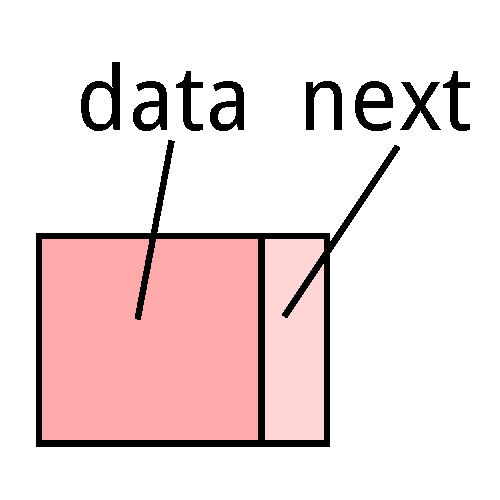
\includegraphics[width=2 cm]{asset/singly-node.pdf}
\end{figure}

\end{frame}

\begin{frame}
\frametitle{Mengenal Linked List (lanj.)}
\begin{itemize}
  \item \foreignTerm{Pointer}-\foreignTerm{pointer} ini menghubungkan antar \foreignTerm{node} dalam \foreignTerm{linked list}.
  \item \foreignTerm{Node} paling depan biasa disebut \alert{\foreignTerm{head}}.
\end{itemize}
\begin{figure}
  \centering 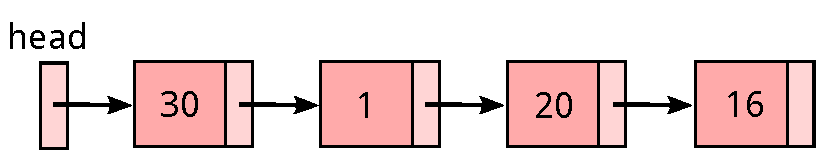
\includegraphics[width=8 cm]{asset/singly-linked-list.pdf}
\end{figure}
\end{frame}

\begin{frame}
\frametitle{Jenis Linked List}
Berdasarkan hubungannya dengan \foreignTerm{node} lain, \foreignTerm{linked list} terbagi menjadi 2 macam, yaitu:
\begin{itemize}
  \item \foreignTerm{singly linked list}: tiap \foreignTerm{node} hanya memiliki \foreignTerm{pointer} ke \foreignTerm{node} selanjutnya saja (next).
  \item \foreignTerm{doubly linked list}: tiap \foreignTerm{node} memiliki \foreignTerm{pointer} ke \foreignTerm{node} selanjutnya (next) dan \foreignTerm{node} sebelumnya (prev).
  \newline
\end{itemize}
Pada pembahasan ini, kita akan menggunakan \foreignTerm{doubly linked list}.
\end{frame}

\begin{frame}
\frametitle{Struktur \foreignTerm{Doubly Linked List}}
\begin{figure}
  \centering
  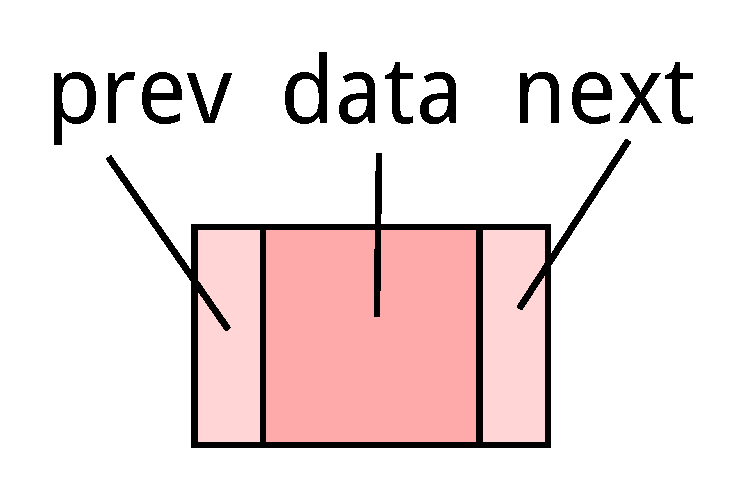
\includegraphics[width=3 cm]{asset/doubly-node.pdf}
\end{figure}
\begin{figure}
  \centering
  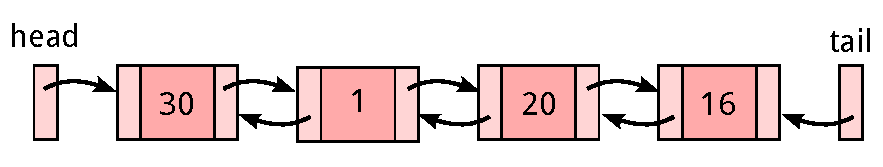
\includegraphics[width=9 cm]{asset/doubly-linked-list.pdf}
\end{figure}
\end{frame}

\begin{frame}
\frametitle{Linked List dan Array}
\begin{itemize}
  \item Pada \foreignTerm{doubly linked list}, biasanya kita hanya memiliki referensi ke \foreignTerm{head} dan \foreignTerm{tail}.
  \item Untuk mengakses elemen ke-$x$ dari \foreignTerm{linked list}, kita dapat melakukannya dengan:

  \begin{codebox}
  \Procname{$\proc{get}(head, x)$}
  \li $current \gets head$
  \li \For $i \gets 2$ \To $x$ \Do
  \li   $current \gets current.next$
      \End
  \li \Return $current$
  \zi
  \end{codebox}
  \item Terlihat tidak efisien?
\end{itemize}
\end{frame}

\begin{frame}
\frametitle{Linked List dan Array (lanj.)}
\foreignTerm{Doubly linked list} memiliki keuntungan dalam:
\begin{itemize}
  \item Menyisipkan elemen baru.
  \item Menghapus suatu elemen.
  \newline
\end{itemize}
Kedua operasi tersebut dapat dilakukan secara efisien.
\end{frame}

\begin{frame}
\frametitle{Menyisipkan Elemen Linked List}
Diberikan $node$ yang bukan $tail$, sisipkan $newNode$ sesudahnya.
\begin{figure}
  \centering
  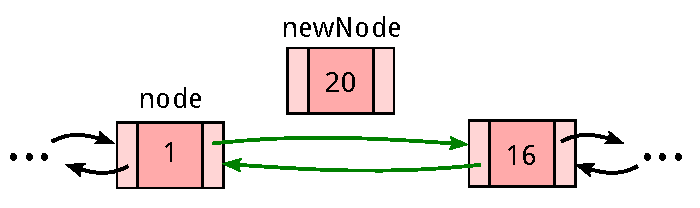
\includegraphics[width=9 cm]{asset/doubly-insert-1.pdf}
\end{figure}
\end{frame}

\begin{frame}
\frametitle{Menyisipkan Elemen Linked List (lanj.)}
1. Isi \foreignTerm{pointer} $newNode.prev$ untuk mengarah ke $node$.

2. Isi \foreignTerm{pointer} $newNode.next$ untuk mengarah ke $node.next$.
\begin{figure}
  \centering
  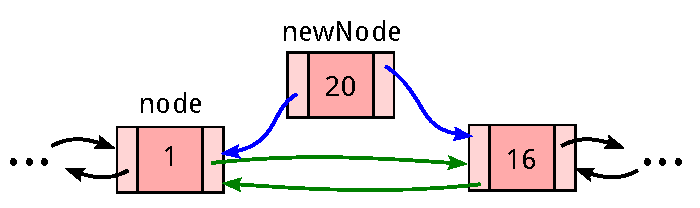
\includegraphics[width=9 cm]{asset/doubly-insert-2.pdf}
\end{figure}
\end{frame}

\begin{frame}
\frametitle{Menyisipkan Elemen Linked List (lanj.)}
3. Perbaiki \foreignTerm{pointer} $newNode.prev.next$ untuk mengarah ke $newNode$.

4. Perbaiki \foreignTerm{pointer} $newNode.next.prev$ untuk mengarah ke $newNode$.
\begin{figure}
  \centering
  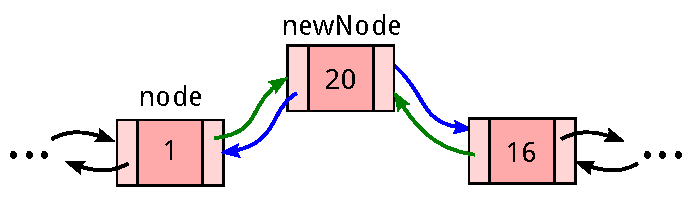
\includegraphics[width=9 cm]{asset/doubly-insert-3.pdf}
\end{figure}
\end{frame}

\begin{frame}
\frametitle{Menyisipkan Elemen Linked List (lanj.)}
\begin{itemize}
  \item Untuk menyisipkan elemen di paling awal atau paling akhir, gunakan cara serupa.
  \item Tidak ada pergeseran, hanya "cabut" dan "pasang" \foreignTerm{pointer}.
  \item Kompleksitasnya adalah $O(1)$.
\end{itemize}
%\begin{codebox}
%\Procname{$\proc{insertAfter}(node, newNode)$}
%\li $newNode.prev \gets node$
%\li $newNode.next \gets node.next$
%\li $newNode.prev.next \gets newNode$
%\li $newNode.next.prev \gets newNode$
%\end{codebox}
\end{frame}

\begin{frame}
\frametitle{Menghapus Elemen Linked List}
Diberikan $node$ yang bukan $head$ maupun $tail$, hapus dari \foreignTerm{linked list}.
\begin{figure}
  \centering
  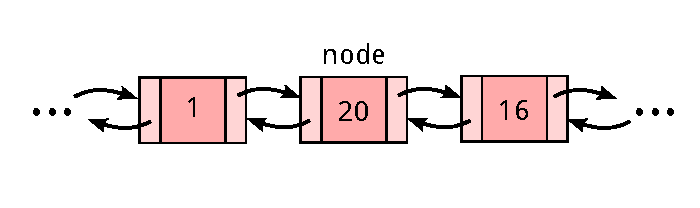
\includegraphics[width=9 cm]{asset/doubly-delete-1.pdf}
\end{figure}
\end{frame}

\begin{frame}
\frametitle{Menghapus Elemen Linked List (lanj.)}
1. Ubah $node.prev.next$ menjadi $node.next$.

2. Ubah $node.next.prev$ menjadi $node.prev$.
\begin{figure}
  \centering
  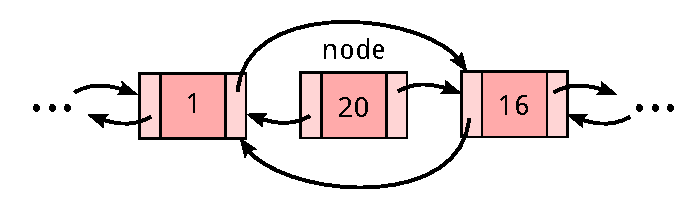
\includegraphics[width=9 cm]{asset/doubly-delete-2.pdf}
\end{figure}
\end{frame}

\begin{frame}
\frametitle{Menghapus Elemen Linked List (lanj.)}
3. Hapus $node$.
\begin{figure}
  \centering
  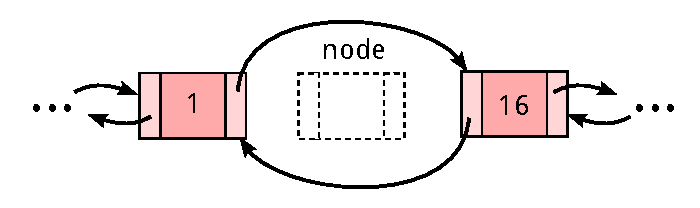
\includegraphics[width=9 cm]{asset/doubly-delete-3.pdf}
\end{figure}
\end{frame}

\begin{frame}
\frametitle{Menghapus Elemen Linked List (lanj.)}
%\begin{codebox}
%\Procname{$\proc{delete}(node)$}
%\li $node.prev.next \gets node.next$
%\li $node.next.prev \gets node.prev$
%\end{codebox}
\begin{itemize}
  \item Anda juga dapat menghapus $head$ atau $tail$ dengan cara serupa.
  \item Sama seperti menyisipkan elemen, tidak ada operasi pergeseran di sini.
  \item Kompleksitasnya adalah $O(1)$.
\end{itemize}
\end{frame}

\begin{frame}
\frametitle{Rangkuman}
\begin{itemize}
  \item \foreignTerm{Linked list} memang tidak mendukung \foreignTerm{random access} secara efisien.
  \item Namun \foreignTerm{linked list} mendukung operasi menyisipkan dan menghapus \emp{jika diketahui} $node$ tempat penyisipan/penghapusan dilakukan.
\end{itemize}
\end{frame}

\section{Stack}

\begin{frame}
\frametitle{Mengenal Stack}
\begin{itemize}
  \item \foreignTerm{Stack} dapat dimisalkan seperti tumpukan piring pada umumnya.
  \item Jika terdapat piring baru yang ingin dimasukkan, maka piring tersebut masuk dari paling atas.
  \item Jika sebuah piring akan diambil dari tumpukan, maka yang diambil juga piring yang paling atas.
\end{itemize}

\begin{figure}
  \centering
  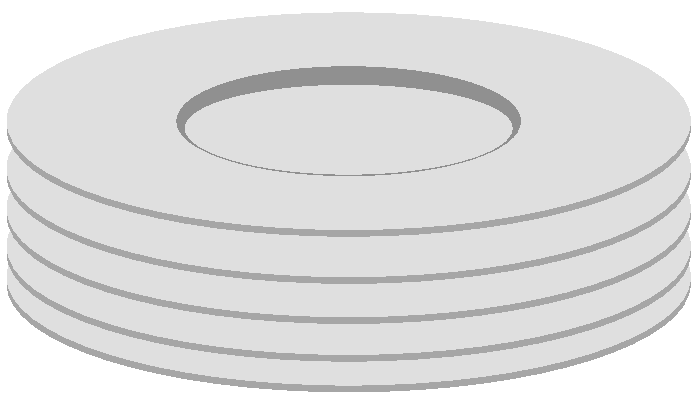
\includegraphics[width=4 cm]{asset/plates-stack.pdf}
\end{figure}
\end{frame}

\begin{frame}
\frametitle{Mengenal Stack (lanj.)}
\begin{itemize}
  \item Struktur data \foreignTerm{stack} menyimpan informasi dalam bentuk tumpukan.
  \item Informasi yang baru dimasukkan ke paling atas tumpukan.
  \item Hanya informasi paling atas yang bisa diakses/dihapus pada setiap waktunya.
  \item Oleh karena itu struktur data \foreignTerm{stack} disebut memiliki sifat LIFO (Last In First Out).
\end{itemize}
\begin{figure}
  \centering
  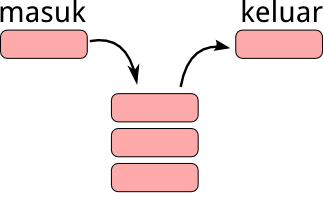
\includegraphics[width=4 cm]{asset/stack.png}
\end{figure}
\end{frame}

\begin{frame}
\frametitle{Operasi pada Stack}

\foreignTerm{Stack} memiliki operasi sebagai berikut:
\begin{itemize}
  \item \foreignTerm{push}, yaitu memasukkan elemen baru ke bagian atas tumpukan.
  \item \foreignTerm{pop}, yaitu membuang elemen paling atas tumpukan.
  \item \foreignTerm{top}, yaitu mengakses elemen paling atas tumpukan.
\end{itemize}
\end{frame}

\begin{frame}
\frametitle{Aplikasi Stack}
\begin{itemize}
  \item Eksekusi fungsi pada sejumlah bahasa pemrograman biasanya menggunakan struktur data \foreignTerm{stack}, tertama untuk fungsi rekursif.
  \item Pemanggilan fungsi rekursif yang menambah kedalaman berarti melakukan "\foreignTerm{push}" pada \foreignTerm{stack} eksekusi fungsi.
  \item Fungsi yang dieksekusi adalah fungsi di paling atas \foreignTerm{stack}.
  \item Setelah fungsi di paling atas selesai, dilakukan "\foreignTerm{pop}" dan eksekusi fungsi dilanjutkan ke fungsi yang ada di paling atas \foreignTerm{stack} berikutnya.
  \item Oleh sebab itu, ketika pemanggilan fungsi terlalu dalam, terjadi \emp{stack overflow}.
\end{itemize}
\end{frame}

\begin{frame}
\frametitle{Aplikasi Stack Lainnya}
\begin{itemize}
  \item \foreignTerm{Stack} juga digunakan pada kalkulator ekspresi matematika dalam notasi \textit{postfix}.
  \item Notasi \textit{postfix} adalah notasi penulisan ekspresi  matematika dengan urutan operand, operand, dan operator.
  \item Contoh:
  \begin{itemize}
    \item "$1 \ 2 \ +$" bermakna "$1 + 2$"
    \item "$1 \ 2 \ 3 + \ -$" bermakna "$1 - (2 + 3)$"
    \item "$1 \ 2 \ 3 + \ - \ 4 \ \times$" bermakna "$(1 - (2 + 3)) \times 4$"
  \end{itemize}
  \item Notasi yang biasa kita gunakan adalah notasi \textit{infix}, yaitu dengan urutan operand, operator, dan operand.
\end{itemize}
\end{frame}

\begin{frame}
\frametitle{Aplikasi Stack Lainnya (lanj.)}
\begin{itemize}
  \item Diberikan sebuah ekspresi dalam notasi \textit{postfix}, nilai akhirnya dapat dicari dengan skema kerja \foreignTerm{stack}.
  \item Pada awalnya, inisialisasi sebuah \foreignTerm{stack} kosong.
  \item Proses ekspresi dari kiri ke kanan:
  \begin{enumerate}
    \item Jika ditemukan operand, \foreignTerm{push} ke dalam \foreignTerm{stack}.
    \item Jika ditemukan operator, \foreignTerm{pop} dua kali untuk mendapat dua operand teratas \foreignTerm{stack}, hitung, lalu \foreignTerm{push} kembali ke dalam \foreignTerm{stack}.
  \end{enumerate}
  \item Satu-satunya nilai terakhir di dalam \foreignTerm{stack} adalah hasil ekspresinya.
\end{itemize}
\end{frame}

\begin{frame}
\frametitle{Eksekusi Ekspresi Postfix}
Ekspresi: $1 \ 2 \ 3 + \ - \ 4 \ \times$
\begin{enumerate}
  \item \foreignTerm{Push} angka 1, \foreignTerm{stack}: [1].
  \item \foreignTerm{Push} angka 2, \foreignTerm{stack}: [1, 2].
  \item \foreignTerm{Push} angka 3, \foreignTerm{stack}: [1, 2, 3].
  \item Ditemukan +:
  \begin{itemize}
    \item \foreignTerm{Pop} dua kali, didapat nilai 2 dan 3, \foreignTerm{stack}: [1].
    \item Operasikan 2 + 3, dan \foreignTerm{push}, \foreignTerm{stack}: [1, 5]
  \end{itemize}
  \item ...
\end{enumerate}
\end{frame}

\begin{frame}
\frametitle{Eksekusi Ekspresi Postfix (lanj.)}
Ekspresi: $1 \ 2 \ 3 + \ - \ 4 \ \times$
\begin{enumerate}
  \setcounter{enumi}{4}
  \item Ditemukan -:
  \begin{itemize}
    \item \foreignTerm{Pop} dua kali, didapat nilai 1 dan 5, \foreignTerm{stack}: [].
    \item Operasikan 1 - 5, dan \foreignTerm{push}, \foreignTerm{stack}: [-4]
  \end{itemize}
  \item \foreignTerm{Push} angka 4, \foreignTerm{stack}: [-4, 4].
  \item Ditemukan $\times$:
  \begin{itemize}
    \item \foreignTerm{Pop} dua kali, didapat nilai -4 dan 4, \foreignTerm{stack}: [].
    \item Operasikan -4 $\times$ 4, dan \foreignTerm{push}, \foreignTerm{stack}: [-16]
    \newline
  \end{itemize}
\end{enumerate}

Jadi  $1 \ 2 \ 3 + \ - \ 4 \ \times = -16$
\end{frame}

\begin{frame}
\frametitle{Implementasi \foreignTerm{Stack}}
\begin{itemize}
  \item Anda dapat mengimplementasikan \foreignTerm{stack} menggunakan \foreignTerm{singly linked list}.
  \item \foreignTerm{Node} yang perlu Anda simpan cukup \foreignTerm{head} saja (atau \foreignTerm{tail} saja), berhubung penyisipan/penghapusan selalu dilakukan di bagian tersebut.
\end{itemize}
\end{frame}

\begin{frame}
\frametitle{Alternatif Implementasi \foreignTerm{Stack}}
\begin{itemize}
  \item Alternatif yang seringkali lebih mudah adalah menggunakan sebuah \foreignTerm{array} dan variabel penunjuk.
  \item Variabel penunjuk ini menyatakan indeks \foreignTerm{array} yang menjadi elemen paling atas \foreignTerm{stack}, dan bergerak maju/mundur sesuai dengan perintah \foreignTerm{push}/\foreignTerm{pop}.
  \item Seluruh operasi dapat dilakukan dalam $O(1)$.
\end{itemize}
\end{frame}

\begin{frame}
\frametitle{Alternatif Implementasi Stack (lanj.)}
\begin{codebox}
\Procname{$\proc{initializeStack}(maxSize)$}
\li \Comment Buat array $stack$ berukuran $maxSize$
\li $topOfStack \gets 0$
\end{codebox}

\begin{codebox}
\Procname{$\proc{push}(item)$}
\li $topOfStack \gets topOfStack + 1$
\li $stack[topOfStack] \gets item$
\end{codebox}

\begin{codebox}
\Procname{$\proc{pop}()$}
\li $topOfStack \gets topOfStack - 1$
\end{codebox}

\begin{codebox}
\Procname{$\proc{top}()$}
\li \Return $stack[topOfStack]$
\end{codebox}

\end{frame}

\begin{frame}
\frametitle{Alternatif Implementasi Stack (lanj.)}
\begin{itemize}
  \item Pastikan nilai $maxSize$ sama dengan maksimal operasi \foreignTerm{push} yang mungkin dilakukan.
  \item Pada operasi \foreignTerm{pop}, kita tidak benar-benar menghapus elemennya, melainkan hanya variabel penunjuknya yang "dimundurkan".
\end{itemize}
\end{frame}

\frame{\sectionpage}

\begin{frame}
\frametitle{Contoh Soal}

\begin{itemize}
  \item Anda diberikan sebuah string, misalnya \texttt{acaabcbcd}.
  \item Cari string \texttt{abc} dalam string tersebut. Jika ditemukan maka hapus string \texttt{abc} tersebut, lalu ulangi pencarian.
  \item Pencarian berakhir ketika tidak terdapat string \texttt{abc} lagi.
  \item Tentukan total penghapusan yang berhasil dilakukan
  \item Contoh, pada string \texttt{acaabcbcd} terdapat sebuah string \texttt{abc}, dan hapus string tersebut menjadi \texttt{acabcd}. Lalu, ditemukan lagi string \texttt{abc} dan hapus menjadi \texttt{acd}. Karena tidak ditemukan lagi string \texttt{abc}, maka jawabannya adalah 2.
\end{itemize}
\end{frame}

\begin{frame}
\frametitle{Pembahasan Soal}

\begin{itemize}
  \item Lakukan iterasi setiap karakter pada string tersebut.
  \item Untuk setiap karakter, \foreignTerm{push} ke dalam \foreignTerm{stack}.
  \item Cek 3 karakter teratas pada \foreignTerm{stack}.
  \item Jika 3 karakter teratas merupakan \texttt{abc}, artinya terdapat 1 penghapusan. Lalu \foreignTerm{pop} ketiga huruf tersebut dari \foreignTerm{stack}.
\end{itemize}
Pada soal ini, Anda harus dapat memodifikasi struktur data \foreignTerm{stack} agar Anda dapat melakukan operasi \foreignTerm{top} pada 3 elemen teratas.

Kompleksitas total adalah $O(N)$, dengan $N$ merupakan panjang string.
\end{frame}

\section{Queue}
\frame{\sectionpage}

\begin{frame}
\frametitle{Mengenal Queue}
\begin{itemize}
  \item Apakah anda pernah melihat antrean pembelian?
  \item Struktur data \foreignTerm{queue} mirip dengan analogi antrean tersebut.
  \item Saat seorang ingin masuk ke antrean, maka orang tersebut harus mengantri dari belakang. \item Sementara itu, orang yang dilayani terlebih dahulu adalah orang yang paling depan.
\end{itemize}
\end{frame}

\begin{frame}
\frametitle{Mengenal Queue (lanj.)}
\begin{itemize}
  \item Struktur data \foreignTerm{queue} menyimpan informasi dalam bentuk antrean.
  \item Informasi yang baru dimasukkan ke paling belakang antrean.
  \item Hanya informasi paling depan yang bisa diakses/dihapus pada setiap waktunya.
  \item Oleh karena itu struktur data \foreignTerm{queue} disebut memiliki sifat FIFO (First In First Out).
\end{itemize}

\begin{figure}
  \centering
  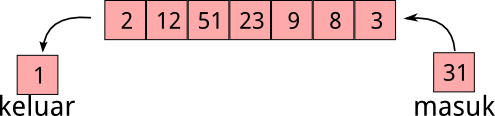
\includegraphics[width=7 cm]{asset/queue.png}
\end{figure}
\end{frame}

\begin{frame}
\frametitle{Operasi Queue}

\foreignTerm{Queue} memiliki beberapa operasi yang dapat dilakukan:
\begin{itemize}
  \item \foreignTerm{push}, yaitu memasukkan elemen baru ke bagian akhir antrean.
  \item \foreignTerm{pop}, yaitu mengeluarkan elemen paling depan antrean.
  \item \foreignTerm{front}, yaitu mengakses elemen yang paling depan antrean.
\end{itemize}
\end{frame}

\begin{frame}
\frametitle{Aplikasi Queue}
\begin{itemize}
  \item Sesuai namanya, pada komputer \foreignTerm{queue} digunakan untuk berbagai hal yang memerlukan antrean.
  \item Misalnya antrean berkas-berkas yang akan diunduh dari internet untuk ditampilkan pada \foreignTerm{browser} Anda.
  \item \foreignTerm{Queue} akan sering kita gunakan ketika sudah memasuki materi graf.
  \item Tepatnya ketika melakukan \foreignTerm{breadth-first search}.
\end{itemize}
\end{frame}

\begin{frame}
\frametitle{Implementasi Queue}
\begin{itemize}
  \item Anda dapat mengimplementasikan \foreignTerm{queue} menggunakan \foreignTerm{singly linked list}.
  \item Anda dapat menyimpan \foreignTerm{node} \foreignTerm{head} dan \foreignTerm{tail}.
  \item Setiap \foreignTerm{push}, sisipkan elemen sesudah \foreignTerm{tail}.
  \item Setiap \foreignTerm{pop}, hapus \foreignTerm{node} \foreignTerm{head}.
\end{itemize}
\end{frame}

\begin{frame}
\frametitle{Alternatif Implementasi Queue}
\begin{itemize}
  \item Lagi-lagi, alternatif yang seringkali lebih mudah adalah menggunakan sebuah \foreignTerm{array} dan dua variabel penunjuk.
  \item Variabel penunjuk ini menyatakan indeks \foreignTerm{array} yang menjadi elemen paling depan dan belakang \foreignTerm{queue}.
  \item Kedua variabel penunjuk ini selalu bergerak maju.
  \item Seluruh operasi dapat dilakukan dalam $O(1)$.
\end{itemize}
\end{frame}

\begin{frame}
\frametitle{Alternatif Implementasi Queue (lanj.)}
\begin{codebox}
\Procname{$\proc{initializeQueue}(maxSize)$}
\li \Comment Buat array $queue$ berukuran $maxSize$
\li $head \gets 1$
\li $tail \gets 0$
\end{codebox}

\begin{codebox}
\Procname{$\proc{push}(item)$}
\li $tail \gets tail + 1$
\li $queue[tail] \gets item$
\end{codebox}

\begin{codebox}
\Procname{$\proc{pop}()$}
\li $head \gets head + 1$
\end{codebox}

\begin{codebox}
\Procname{$\proc{front}()$}
\li \Return $queue[head]$
\end{codebox}
\end{frame}

\begin{frame}
\frametitle{Alternatif Implementasi Queue (lanj.)}
\begin{itemize}
  \item Kelemahan dari implementasi ini adalah beberapa elemen di bagian awal \foreignTerm{array} tidak digunakan kembali.
  \item Misalnya telah dilakukan 15 kali \foreignTerm{push}, dan 11 kali \foreignTerm{pop}.
  \item Sebanyak 11 elemen pertama pada \foreignTerm{array} tidak akan digunakan kembali.
  \item Ini adalah pemborosan, karena aslinya hanya terdapat 4 elemen di dalam \foreignTerm{queue}.
  \item Meskipun demikian, dalam dunia kompetisi hal ini masih dapat diterima.
  \item Pastikan nilai $maxSize$ sama dengan maksimal operasi \foreignTerm{push} yang mungkin dilakukan.
\end{itemize}
\end{frame}

%\section{Binary Search Tree}
%\frame{\sectionpage}
%
%\begin{frame}
%\frametitle{Motivasi}
%\begin{itemize}
%  \item Anda diberikan sejumlah perintah.
%  \item Terdapat 2 macam perintah, yaitu:
%  \begin{enumerate}
%    \item Simpan suatu angka $x$.
%    \item Cari apakah suatu angka $x$ pernah disimpan.
%  \end{enumerate}
%  \item Bagaimana Anda akan menyelesaikan masalah ini?
%\end{itemize}
%\end{frame}
%
%\begin{frame}
%\frametitle{Solusi Sederhana}
%Cara yang paling mudah adalah:
%\begin{itemize}
%  \item Untuk tiap operasi menyimpan, masukkan angka tersebut ke dalam array.
%  \item Untuk operasi cari, lakukan linear search pada array.
%  \newline
%\end{itemize}
%Operasi pencarian ini kurang efisien karena butuh $O(N)$ untuk mencari angka tersebut.
%\end{frame}
%
%\begin{frame}
%\frametitle{Solusi Lainnya}
%Cara lainnya adalah:
%\begin{itemize}
%  \item Untuk tiap operasi menyimpan, masukkan angka tersebut ke dalam array sedemikian sehingga array selalu dalam keadaan terurut.
%  \item Hal ini dapat dilakukan dengan prosedur seperti pada insertion sort.
%  \item Untuk operasi cari, lakukan binary search pada array.
%  \newline
%\end{itemize}
%Namun kini operasi menyimpan menjadi kurang efisien karena butuh $O(N)$ untuk melakukan "insertion" dan menjaga array tetap terurut.
%\end{frame}
%
%\begin{frame}
%\frametitle{Mengenal Binary Search Tree}
%\begin{itemize}
%  \item Untuk menyelesaikan masalah tersebut secara lebih efisien, kita dapat menggunakan Binary Search Tree (BST).
%  \item BST merupakan struktur data yang cukup berbeda dengan struktur data yang sebelumnya kita pelajari.
%\end{itemize}
%
%\begin{figure}
%  \centering
%  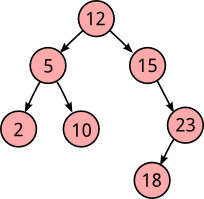
\includegraphics[width=4 cm]{asset/bst.png}
%\end{figure}
%\end{frame}
%
%\begin{frame}
%\frametitle{Mengenal BST (lanj.)}
%Aturan BST:
%\begin{itemize}
%  \item Tiap node pada BST memiliki sebuah nilai dan 2 pointer ke anaknya, yaitu anak kiri dan anak kanan.
%  \item Semua node yang berada di sebelah kiri suatu node pasti memiliki nilai yang lebih kecil daripada node sekarang.
%  \item Semua node yang berada di sebelah kanan suatu node pasti memiliki nilai yang lebih besar daripada node sekarang.
%  \item Node yang paling atas merupakan node \alert{root} yang merupakan satu-satunya node yang dapat diakses secara langsung
%\end{itemize}
%\end{frame}
%
%\begin{frame}
%\frametitle{Operasi Insert pada BST}
%
%Dengan adanya sifat-sifat BST di atas, maka proses insert dapat dimulai dari node root. Lakukan hal berikut hingga menemukan node NULL.
%\begin{itemize}
%  \item Jika nilai pada node sekarang lebih besar daripada nilai yang akan diinsert, maka pergi ke anak kiri dari node sekarang.
%  \item Jika nilai pada node sekarang lebih kecil dari nilai yang akan diinsert, maka pergi ke anak kanan dari node sekarang.\newline
%\end{itemize}
%
%Jika node sekarang NULL, maka buat node baru dengan anak kiri dan anak kanan adalah NULL. Jangan lupa untuk memasukkan nilai yang diinsert ke node tersebut.
%\end{frame}
%
%\begin{frame}[fragile]
%\frametitle{Pseudocode Insert pada BST}
%
%\begin{lstlisting}
%
%node* insert (node* currNode, int value)
%
%    if currNode = NULL:
%        currNode = new Node
%        currNode.val = value
%        currNode.left_child = NULL
%        currNode.right_child = NULL
%
%    else if currNode.val > value:
%        currNode.left_child =
%        insert(currNode.left_child, value)
%
%    else:
%        currNode.right_child =
%        insert(currNode.right_child, value)
%
%    return currNode
%
%\end{lstlisting}
%\end{frame}
%
%\begin{frame}
%\frametitle{Operasi Find pada BST}
%
%Dengan adanya sifat-sifat BST di atas, maka proses find dapat dimulai dari node root. Lakukan hal berikut hingga menemukan angka yang dicari atau menemukan node NULL.
%\begin{itemize}
%  \item Jika nilai pada node sekarang lebih besar daripada nilai yang akan diinsert, maka pergi ke anak kiri dari node sekarang.
%  \item Jika nilai pada node sekarang lebih kecil dari nilai yang akan diinsert, maka pergi ke anak kanan dari node sekarang.\newline
%\end{itemize}
%Jika value dari node sekarang sesuai dengan yang dicari, berarti angka yang dicari ditemukan dalam BST.
%\newline\newline
%Jika node sekarang NULL, maka angka yang dicari tidak ditemukan dalam BST.
%\end{frame}
%
%\begin{frame}[fragile]
%\frametitle{Pseudocode Insert pada BST}
%
%\begin{lstlisting}
%
%int insert (node* currNode, int value)
%
%    if currNode = NULL:
%        return 0
%
%    else if currNode.val = value:
%        return 1
%
%    else if currNode.val > value:
%        return insert(currNode.left_child, value)
%
%    else:
%        return insert(currNode.right_child,value)
%
%\end{lstlisting}
%\end{frame}
%
%\begin{frame}
%\frametitle{Pembahasan Soal}
%
%Setelah mengenai BST, maka untuk menyelesaikan masalah sebelumnya kita dapat menggunakan BST. Untuk proses insert, maka gunakan proses insert yang terdapat pada BST. Untuk proses find, juga gunakan proses find yang terdapat pada BST.
%\newline\newline
%Dengan demikian, kompleksitas dari insert dan find keduanya adalah sesuai dengan tinggi dari BST. Solusi ini lebih efisien daripada menggunakan array dan harus mencari seluruh isi array
%\end{frame}

\begin{frame}
\frametitle{Penutup}
\begin{itemize}
  \item Struktur data yang baru kita pelajari ini merupakan struktur data dasar.
  \item Pada lain kesempatan, kita akan mempelajari struktur data yang lebih kompleks dan manfaatnya lebih "berasa", seperti \foreignTerm{heap} untuk \foreignTerm{priority queue}, \foreignTerm{binary search tree} untuk kamus, dan \foreignTerm{segment tree} untuk \foreignTerm{dynamic range query}.
\end{itemize}
\end{frame}

\end{document}


